\documentclass[]{kththesis}

\usepackage{amsmath}
\usepackage{amsfonts}
\DeclareMathOperator{\Lapl}{\mathcal{L}}
\DeclareMathOperator{\bigO}{\mathcal{O}}
\DeclareMathOperator{\Real}{\mathbb{R}}

\newif\ifthesis
\thesistrue

\usepackage[bottom]{footmisc}

\usepackage[backend=bibtex, style=numeric, sorting=none]{biblatex}
\addbibresource{references.bib}

\usepackage{graphicx}
\usepackage{caption}
\usepackage{subcaption}
\usepackage{float}
\usepackage{pgfplots}
\usepgfplotslibrary{groupplots}

\usepackage{algorithm}
\usepackage{algorithmic}
\renewcommand{\algorithmicrequire}{\bf{Input:}}
\renewcommand{\algorithmicensure}{\bf{Output:}}

\usepackage{enumitem}
\usepackage{hyperref}

\title{Image Processing using Graph Laplacian Operator}
\alttitleSW{Bildbehandling med graf Laplaceoperatorn}
\alttitleFR{Traitement d'image en utilisant le Laplacien de graphe}

\author{David Wobrock}
\email{david.wobrock@gmail.com}
\date{\today}
\programme{Master Thesis in Computer Science}

\supervisor{Frédéric Nataf}
\team{ALPINES Team - INRIA Paris}

\supervisorKTH{Stefano Markidis}
\examinerKTH{Erwin Laure}
\schoolKTH{School of Computer Science and Communication - KTH}

\supervisorINSA{Christine Solnon}
\schoolINSA{Département Informatique - INSA de Lyon}

\begin{document}

\frontmatter % includes the titlepage, abstracts and table of contents

\titlepage

\begin{abstract}
 The latest image processing methods are based on global data-dependent filters.
These methods involve huge affinity matrices which cannot fit in memory and need to be approximated using spectral decomposition.
The inferred eigenvalue problem concerns the smallest eigenvalues of the Laplacian operator which can be solved using the inverse iteration method which, in turn, involves solving linear systems.
In this master thesis, we detail the functioning of the spectral algorithm for image editing and explore the behaviour of solving large and dense systems of linear equations in parallel, in the context of image processing.
We use Krylov type solvers, such as GMRES, and precondition them using domain decomposition methods to solve the systems on high-performance clusters.
The experiments show that Schwarz methods as preconditioner scale well as we increase the number of processors.
However, we observe that the limiting factor is the Gram-Schmidt orthogonalisation procedure.
We also compare the performances to the state-of-the-art Krylov-Schur algorithm provided by the SLEPc library.

\end{abstract}

\begin{otherlanguage}{swedish}
  \begin{abstract}
   Svenska abstract går här.

  \end{abstract}
\end{otherlanguage}

\begin{otherlanguage}{french}
  \begin{abstract}
   Les plus récentes méthodes de traitement d'images sont basées sur des filtres globaux dépendant des données.
Ces méthodes impliquent d'immenses matrices de similarités et de Laplacien de graphe de l'image en entrée.
Puisque ces matrices ne tiennent pas en mémoire, il est nécessaire de les approcher par l'échantillonnage et l'extension de Nystr\"om basée sur la décomposition spectral des matrices.
Le problème aux valeurs propres qui en découle concerne les plus grandes valeurs propres du filtre.
Néanmoins, celle-ci corresponde aux plus petites valeurs propres du Laplacien.
Pour résoudre ce problème, nous utilisons la méthode la puissance inverse, qui converge mieux dans ce cas, mais qui implique la résolution de systèmes linéaires.
Dans cette thèse de master, nous étudions le comportement de la résolution de systèmes d'équations linéaires sur de grandes matrices pleines, dans le cadre du traitement d'images, en utilisant des méthodes de décomposition de domaines comme préconditionneur.
Les expériences montrent que les méthodes de type Krylov combinées avec les méthodes de Schwarz comme préconditionneur passe bien à l'échelle pour de grandes systèmes linéaires avec des matrices pleines.

  \end{abstract}
\end{otherlanguage}

\tableofcontents

\mainmatter % Thesis content

\chapter{Introduction}

\section{Background}

\paragraph{}
The talk \cite{siam_slides_2016} and articles \cite{glide_2014} \cite{talebi_nonlocal_2014} by Milanfar, working at Google Research, about using the graph Laplacian operator for nonconformist image processing purposes awakes curiosity.

Indeed, Milanfar reports that these techniques to build image filters are used on smartphones, which implies a reasonable execution time with limited computational resources.
Over 2 billion photos are shared daily on social media \cite{siam_slides_2016}, with very high resolutions and most of the time some processing or filter is applied to them.
The algorithm must be efficient to be deployed at such scale.

\section{Objective}

\paragraph{}
The aim of this degree project is not to explore and improve the state of image processing.
Instead, the spectral methods used in the algorithm will be our focus point.
Those will inevitably expose eigenvalue problems, which may involve solving systems of linear equations.

Concerning the challenges about solving linear systems, on one hand, the size of the systems can be large considering high-resolution images with millions of pixels, or even considering 3D images.
We handle huge matrices of size \(N^2\), with \(N\) the number of pixels of the input image.
On the other hand, images are dense matrices and so will be the matrices we compute, thus also the exposed linear systems.
Often, linear systems result from discretising partial differential equations yielding sparse matrices, and therefore most linear solvers are specialised in sparse systems.

We want to explore the performance of linear solvers on dense problems, their stability and convergence.
This will include preconditioning the linear systems, especially using domain decomposition methods, and analyse their behavior on dense systems.

\section{Related work}

\paragraph{}
In this section, we start by a summary of spectral graph theory as an introduction to the project.
It is followed by image processing techniques for denoising, with traditional patch-based methods and global image filters.
And we finish by a quick overview of linear solvers.

\subsection{Spectral graph theory}

\paragraph{}
Spectral graph theory has a long history starting with matrix theory and linear algebra that were used to analyse adjacency matrices of graphs.
It consists in studying the properties of graphs in relation to the eigenvalues and eigenvectors of the adjacency or Laplacian matrix.
The eigenvalues of such a matrix are called the spectrum of the graph.
The second smallest eigenvalue has been called ``algebraic connectivity of a graph" by Fiedler \cite{fiedler_algebraic_1973}, and is therefore also known as \textit{Fiedler value}, because it contains interesting information about the graph.
Indeed, it can show if the graph is connected, and by extending this property, we can count the number of connected components in the graph through the eigenvalues of the graph Laplacian and do graph partitioning.

The field of spectral graph theory is very broad and the eigendecomposition of graphs is used in a lot of areas.
Spectral graph theory has many applications such as graph colouring, graph isomorphism testing, random walks and graph partitioning among others.

One of the most complete works about spectral graph theory is \cite{chung_spectral_1997} by Fan Chung.
This monograph exposes many properties of graphs, the power of the spectrum and how spectral graph theory links the discrete world to the continuous one.

\paragraph{Laplacian matrix}
Since the adjacency matrix of a graph only holds basic information about it, we usually augment it to the Laplacian matrix.
Multiple definitions of the Laplacian matrix are given in \cite{chung_spectral_1997} and \cite{siam_slides_2016}, and each one has different properties.
The most common ones are the normalised Laplacian and the Random Walk Laplacian.
However, more convenient formulations, like the ``Sinkhorn" Laplacian \cite{milanfar_symmetrizing_2013} and the re-normalised Laplacian \cite{siam_slides_2016} \cite{milanfar_new_2016}, have been proposed since.

\paragraph{The Spectral Theorem}
Some Laplacian definitions result in a symmetric matrix, which is a property that is particularly interesting for spectral theory because of the Spectral Theorem \cite{zhang_spectral_2010}.
Let \(S\) be a real symmetric matrix of dimension \(n\), \(\Phi = [\phi_1 \phi_2 \dots \phi_n ]\) the matrix of eigenvectors of \(S\) and \(\forall i \in [0,n]\), let \(\Pi = diag\{\lambda_i\}\) the diagonal matrix of the eigenvalues of \(S\), then
\[S = \Phi \Pi \Phi^T = \sum_{i=1}^n \lambda_i \phi_i \phi_i^T,\]
the eigendecomposition of \(S\).
We note that the eigenvalues of \(S\) are real and that the eigenvectors are orthogonal, i.e., \(\Phi^T\Phi = I\), with \(I\) the identity matrix.

%\paragraph{Cheeger's inequality}
%One of the most fundamental theorems of spectral graph theory concerns the Cheeger's inequality and Cheeger constant.
%It approximates the sparsest cut of a graph with the second eigenvalue of its Laplacian.
%
%The Cheeger constant \cite{cheeger_lower_1969} measures the degree of ``bottleneck" of a graph, useful for constructing well-connected graphs.
%Considering a graph \(G\) of \(n\) vertices, the Cheeger constant \(h\) is defined as
%\[h(G) = min_{0 < |S| \le \frac{n}{2}} \frac{|\partial S|}{|S|},\]
%where \(S\) is a subset of the vertices of \(G\) and \(\partial S\) is the \textit{edge boundary} of \(S\) to have all edges with exactly one endpoint in \(S\), or formally
%\[\partial S = {{u, v} \in V(G) : u \in S, v \notin S},\]
%with \(V(G)\) the vertices of graph \(G\).
%
%Cheeger's inequality defines a bound and relationship on the smallest positive eigenvalue of the Laplacian matrix \(\Lapl \) such as
%\[\lambda_1(\Lapl) \ge \frac{h^2(\Lapl)}{4}.\]
%
%When the graph \(G\) is \(d\)-regular, thanks to \cite{cvetkovic_spectra_1980}, we also have an inequality between \(h(G)\) and the second smallest eigenvalue \(\lambda_2\) such as
%\[\frac{1}{2}(d-\lambda_2) \le h(G) \le \sqrt{2d(d-\lambda_2)},\]
%where \(d - \lambda_2\) is also called the \textit{spectral gap}.

\paragraph{}
The Laplacian is the foundation of the heat equation, fluid flow and essentially all diffusion equations.
It can generally be thought that the Laplacian operator is a center-surround average \cite{siam_slides_2016} of a given point.
Therefore, applying it on an image results in smoothing.
Generally, applying the graph Laplacian operator on an image provides useful information about it and enables possibilities of interesting image processing techniques.

\subsection{Image processing - denoising}

\paragraph{Background}
Even with high quality cameras, denoising and improving a taken picture remains important.
The two main issues that have to be addressed by denoising are blur and noise.
The effect of blur is internal to cameras since the number of samples of the continuous signal is limited and it should hold the Shannon-Nyquist theorem \cite{buades_review_2005}, stipulating a sufficient condition on the number of samples required to discretise a countinous signal without losing information.
Noise comes from the light acquisition system that fluctuates in relation to the amount of incoming photons.

To model these problems, a classical approach to formulate the deficient image considers \(z\) the clean signal vector, \(e\) a noise vector of variance \(\sigma^2\) and \(y\) the noisy picture:
\[y = z + e.\]

What we want is a high-performance denoiser, capable of scaling up in relation to increasing the image size and keeping reasonable performances.
The output image should come as close as possible to the clean image.
As an important matter, it is now generally accepted that images contain a lot of redundancy.
This means that, in a natural image, every small enough window has many similar windows in the same image.

\paragraph{Traditional, patch-based methods}
The image denoising algorithms review proposed by \cite{buades_review_2005} suggests that the non-local means algorithm, compared to other reviewed methods, comes closest to the original image when applied to a noisy image.
This algorithm takes advantage of the redundancy of natural images and for a given pixel predicts its value by using the pixels in its neighbourhood.

In \cite{dabov_image_2007}, the authors propose the BM3D algorithm, a denoising strategy based on grouping similar 2D blocks of the image into 3D data arrays.
Then, collaborative filtering is performed on these groups and return 2D estimates of all grouped blocks.
This algorithm exposed state-of-the-art performance in terms of denoising at that time.
The results are still one of the best for a reasonable computational cost.

\paragraph{Global filter}
In the last couple of years, global image denoising filters came up, based on spectral decompositions \cite{glide_2014}.
This approach considers the image as a complete graph, where the filter value of each pixel is computed by all pixels in the image.
We define the result image \(z\), \(W\) the huge data-dependent global filter of size \(N \times N\), with \(N\) the number of pixels and the input image \(y\):
\[z = Wy.\]
To show an example of the size of the filter, a standard 10 MPixel picture will result in a filter matrix of \(10^{14}\) elements, taking 800 TB of memory.
This kind of filter is considered in this report.

Those huge matrices will need to be approximated using their eigendecomposition.
And these will need to solve systems of linear equations.

\subsection{Linear solvers and domain decomposition methods}

\paragraph{}
Solving a system of linear equations such that
\[Ax = b,\]
is often critical in scientific computing.
When discretising equations coming from physics for example, a huge linear system can be obtained.
Multiple methods exist to solve such systems, even when the system is large and expensive to compute.
We present in the following the most used and known solvers.

\paragraph{Direct solvers}
The most commonly used solvers for systems of linear equations are direct solvers.
They provide robust methods and optimal solutions to the problem.
However, they can be hard to parallelise and have difficulties with large input.
The most famous is the backslash operator from MATLAB which performs tests to determine which special case algorithm to use, but ultimately falls back on a LU factorisation \cite{mldivide_matlab}.
The LU factorisation, which is a Gaussian elimination, is hard to parallelise.
Although, a block version of the LU factorisation exists that can be parallelised more easily.
There are other parallel direct solvers, like MUMPS \cite{MUMPS_2001}, but generally they reach their computational limit above \(10^6\) degrees of freedom in a 2D problem, and \(10^5\) in 3D.

\paragraph{Iterative solvers}
For larger problems, iterative methods must be used to achieve reasonable runtime performances.
The two types of iterative solvers are fixed-point iteration methods and Krylov type methods.
Both require only a small amount of memory and can often be parallelised.
The main drawback is that these methods tend to be less robust than direct solvers and convergence depends on the problem.
Indeed, ill-conditioned input matrices will be difficult to solve correctly by iterative methods and do not necessarily converge.
Generally, Krylov methods are preferred over fixed-point iteration methods.
The most relevant iterative Krylov methods are the Conjugate Gradient (CG) and the Generalised Minimal Residual method (GMRES) \cite{saad_iterative_2003} \cite{saad_gmres_1986}.

To tackle the ill-conditioned matrices problem, there is a need to precondition the system.


\paragraph{Preconditioners - Domain decomposition methods}
One of the ways to precondition systems of linear equations is to use domain decomposition.
The idea goes back to Schwarz who wanted to solve a Poisson problem on a complex geometry.
He decomposed the geometry into multiple smaller simple geometric forms, making it easy to work on subproblems.
This idea has been extended and improved to propose fixed-point iterations solvers for linear systems.
However, Krylov methods expose better results and faster convergence, but domain decomposition methods can actually be used as preconditioners to the system.
Famous Schwarz preconditioners are the Restricted Additive Schwarz method (RAS) and the Additive Schwarz Method (ASM).
With \(M^{-1}\) the preconditioning matrix, we shall solve
\[M^{-1}Ax = M^{-1}b\]
which exposes the same solution as the original problem.

\paragraph{}
Domain decomposition methods will also be an important topic of this degree project.
These methods are usually applied to solve problems of linear algebra involving partial differential equations (PDEs).
Solving the discretised problem leads to solving linear systems.

Our main reference will be \cite{dolean_domain_2015} which focuses on the parallel linear iterative solvers for systems of linear equations.
Domain decomposition methods are naturally parallel which is convenient for the current state of processor progress.
Without going into the details, we will make use of Schwarz methods for preconditioning and iterative Krylov subspace methods as solvers.

\section{Delimitations}

\paragraph{}
TODO

\section{Outline}

\paragraph{}
The document is organised in the following way.
Chapter 2 introduces the global filter algorithm that has been explored during this project.
It explains the image processing method in a general way and then clarifies the variations that can be used.
It serves as a reference to understand the algorithm and the problems that arise.
Chapter 3 shows the work that has been done on the implementation side.
It explains the used parallelism and exposes experimental results of this approach.


\chapter{Image processing using the graph Laplacian operator}

\paragraph{}
Multiple image processing filters can be built using the graph Laplacian operator.
As Milanfar mentions in \cite{siam_slides_2016}, smoothing, deblurring, sharpening, dehazing, and other filters can be created.
Laplacian operators can also be used as the basis for compression artifact removal, low-light imaging and image segmentation.

We shall consider an adapted version of the proposed algorithm in \cite{glide_2014} to solve the eigenvalue problem by solving linear systems.
Let's introduce step-by-step the algorithm and how we consider it.

\section{Algorithm}

\paragraph{}
An image filter consists of a function which outputs one pixel, taking all pixels as input and applying weights to them. We can write this as
\[z_i = \sum_j W_{ij}y_j,\]
\(z_i\) being the output pixel, \(W_{ij}\) the weight and \(y_j\) all input pixels.
This means that a vector of weights exists for each pixel.

So, as a practical notation, we can say that, with \(W\) the matrix of weights and \(y\) the input image as a vector,
\[z = Wy.\]
The filter matrix \(W\) considered here is data-dependent and built upon the input image \(y\).

\paragraph{Image as graph}
Let's think of an image as a graph.
Each pixel is a node and has edges to other nodes.
The simplest way to connect pixels to other pixels is their direct neighbours, in which case each node has four edges.
To avoid losing any information, we will instead consider the case of a complete graph, each node connects to all other nodes.

To preserve the image information in the graph, the graph edges will be assigned a weight, measuring the similarity\footnote{Also called affinity.} between the two nodes, thus between two pixels.
There are multiple ways the similarity can be defined.

The most intuitive definition considers spatial proximity.
This means that similar pixels are spatially close, which, translated to a basic filter, is the same as a Gaussian filter which computes a weighted average of the pixel's neighbourhood and produces what is known as Gaussian blur.
Another similarity definition is to consider the pixel's color.
A good compromise is to consider an average of both, spatial and color closeness, with a certain weighting.

From this definition can be computed the adjacency matrix of the graph taking into account the edge weights.
We will call this matrix the affinity matrix\footnote{Or similarity matrix or kernel matrix}\ \(K\) which represents the similarity of each pixel to every other pixel in the image.
Consequently, this matrix is symmetric and of size \(N \times N\) with \(N\) the number of pixels in the image, and, depending on the similarity function, its values \(0 \le K_{ij} \le 1\).

Using this affinity matrix, we obtain the graph Laplacian \(\Lapl\), used to build the filter matrix \(W\).

\paragraph{Building the filter}

Multiple graph Laplacian definitions, more or less equivalent, exist and can have slightly different properties.
In the case of image smoothing, the filter \(W\) is defined such as \(\Lapl = I - W\) \cite{siam_slides_2016} and so \(W = I - \Lapl\).

However, all these matrices \(K\), \(\Lapl\) and \(W\) represent huge computational costs.
Only storing one of these matrices is already a challenge since they have a size of \(N^2\).

For example, a tiny test image of size \(256 \times 256\) has 65 536 pixels, so one of these matrices has approximately \(4.29 \times 10^9\) elements.
Considering storing those with a 64 bits type, one matrix takes more than 34 GB of memory.
Scaling to an everyday-smartphone picture, taken with a 10 MPixel camera, a matrix contains \(10^{14}\) elements, meaning a 800 TB matrix.

\paragraph{Approximation by sampling and Nystr\"om extension}

To avoid storing any of those huge matrices, approximation will be necessary.
It starts by sampling the image and only select a subset of \(p\) pixels, with \(p \ll N\).
Numerically, \(p\) should represent around 1\% of the image pixels.
The rows and columns of the matrix \(K\) are re-organised such as
\[K = \begin{bmatrix}K_A & K_B \\ K_B^T & K_C\end{bmatrix}\]
with \(K_A\) being the affinities between the sampled pixels and thus of size \(p \times p\).
\(K_B\) holds the affinities between the sampled pixels and the remaining pixels and is therefore of size \(p \times (N-p)\).
Finally, the submatrix \(K_C\) contains the similarities between the remaining pixels.
Knowing that \(K_C\) is of size \((N-p) \times (N-p)\) and that \(p \ll N\), this submatrix is huge.

To have a numerical approximation of a symmetric matrix \(K\), we use the eigendecomposition:
\[K = \Phi \Pi \Phi^T\]
where \(\Phi\) are the orthonormal eigenvectors of \(K\) stored as a matrix and \(\Pi\) contains the eigenvalues of \(K\).
\cite{fowlkes_spectral_2004} suggests the Nystr\"om extension to approximate \(K\) by \(\tilde{K} = \tilde{\Phi} \tilde{\Pi} \tilde{\Phi^T}\), with \(\tilde{\Pi} = \Pi_A\) and the first \(p\) eigenvectors:
\[\tilde{\Phi} = \begin{bmatrix}\Phi_A \\ K_B^T \Phi_A \Pi_A^{-1}\end{bmatrix}\]
with the eigendecomposition \(K_A = \Phi_A \Pi_A \Phi_A^T\).
The approximated matrix would be of the form \cite{glide_2014}
\[\tilde{K} = \begin{bmatrix}K_A & K_B \\ K_B^T & K_B^T K_A^{-1} K_B\end{bmatrix}.\]
We can clearly see that the huge submatrix \(K_C\) is now approximated.

\paragraph{Eigendecomposition}
We need to compute the largest eigenvalues of the filter.
For the approximation, we will actually need to compute the largest eigenvalues of the sampled pixels of the filter to use the Nystr\"om extension.
We know that the eigenvalues of submatrix\ \(K_A\) are between the extremum eigenvalues of the filter, which is known as the interlacing property of principal submatrices.
We also know that computing the largest eigenvalues of the submatrix filter is equivalent to computing the smallest eigenvalues of the corresponding submatrix of the Laplacian operator.
The proofs to these statements can be found in Appendix \ref{appendix:eigenvalue_proof}.

The goal of this observation is the way of computing the eigenvalues.
For the largest eigenvalues, the most famous algorithm is the power method.
For the smallest eigenvalues, the inverse power method is usually used.
The latter requires either to invert a matrix, or to solve a linear system.
We will solve systems of linear equations to compute the first eigenvalues of the Laplacian in order to observe the behavior of solvers on the dense matrices.

So our approximated Laplacian eigendecomposition, using the Nystr\"om extension and eigendecomposition of \(\Lapl_A\):
\[\tilde{\Lapl} = \tilde{\Phi} \tilde{\Pi} \tilde{\Phi^T}.\]

\paragraph{Output image}
\cite{modern_tour_2013} defines the filter as \(W = I - \Lapl\) and therefore the output image using the filter approximation can be expressed as:
\begin{equation}
 \begin{split}
     \tilde{z} & = \tilde{W}y \\
               & = (I - \tilde{\Lapl}) y \\
               & = (I - \tilde{\Phi} \tilde{\Pi} \tilde{\Phi^T}) y \\
               & = y - \tilde{\Phi} \tilde{\Pi} \tilde{\Phi^T} y
 \end{split}
\end{equation}

\begin{algorithm}[H]
 \caption{Image processing using graph Laplacian operator}
 \begin{algorithmic}
  \REQUIRE \(y\) an image of size \(n \times m\)
  \ENSURE \(z\) the output image
  \STATE \(N \leftarrow n*m\)
  \STATE \COMMENT{Sampling}
  \STATE Sample \(p\) pixels, \(p \ll N\)
  \STATE \COMMENT{Kernel matrix approximation}
  \STATE Compute \(K_A\) (size \(p \times p\)) and \(K_B\) (size \(p \times (N-p)\)) such as \(K = \begin{bmatrix} K_A & K_B \\ K_B^T & K_C \end{bmatrix}\)
  \STATE Compute the Laplacian \(\Lapl_A\) and \(\Lapl_B\)
  \STATE \COMMENT{Eigendecomposition}
  \STATE Compute the smallest eigenvalues \(\Pi_A\) and the associated eigenvectors \(\Phi_A\) of \(\Lapl_A\)
  \STATE Nystr\"om extension \(\tilde{\Phi} \leftarrow \begin{bmatrix} \Phi_A \\ \Lapl_B^T \Phi_A \Pi_A^{-1} \end{bmatrix}\)
  \STATE \COMMENT{Apply the filter}
  \STATE \(\tilde{z} \leftarrow y - \tilde{\Phi} \tilde{\Pi} \tilde{\Phi^T} y\)
 \end{algorithmic}
\end{algorithm}

\section{Variations}

\subsection{Sampling method}

\paragraph{}
The sample requires to represent only less than 1\% of the pixels of the image \cite{glide_2014}.
To achieve this, we can use different approaches. The chosen method is decisive for the application of the Nystr\"om method.
\begin{description}[align=left]
 \item [Random sampling (RS)] most common and simple sampling scheme, but no deterministic guarantee of the output quality. It can produce good results for images with poor resolution, but with a huge amount of data, random sampling is limited because it cannot reflect the structure of the data set \cite{zhan_improved_2017}.
 \item [K-means sampling (KS)] associate to each pixel a 5-D space (R, G, B, X, Y) and divide the pixels into K clusters (K centers). These clusters are a good sampling scheme for images with simple and uniform backgrounds \cite{kao_sampling_2012} \cite{zhang_improved_2008}.
 \item [Uniform spatially sampling] the uniformity of the sample gives good results for image sampling because of the spatial correlation of pixels. This method remains simple but effective \cite{glide_2014}.
  \begin{figure}[H]
      \centering
      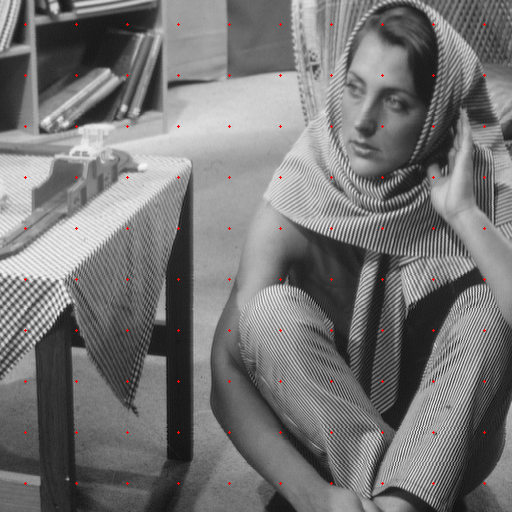
\includegraphics[width=0.6\textwidth]{img/spatiallyUniformSampling.png}
      \caption{Spatially uniform sampling. Red pixels are sampled. Here 100 pixels are sampled, which only represents 0.04\% of all pixels}
  \end{figure}
 \item [Incremental sampling (INS)] is an adaptive sampling scheme, meaning that it select points according to the similarity, so that we can have an approximate optimal rank-k subspace of the original image \cite{zhan_improved_2017}.
 \item [Mean-shift segmentation-based sampling] this scheme performs good for complex backgrounds. The method consists in over-segmenting the image into \(n\) regions and only one pixel of each region will be sampled using the spatially closest pixel to the center of the region given a formula in \cite{kao_sampling_2012}.
\end{description}

\subsection{Affinity function}

\paragraph{}
The kernel function \(\mathcal{K}_{ij}\) measures the similarity between the pixel \(y_i\) and \(y_j\).
The chosen function is important because it decides on which features the similarity of pixels will be evaluate and the tolerance of it.
Some of the most used affinity functions are:

\begin{description}[align=left]
 \item [Spatial Gaussian Kernel] takes only into account the spatial distance between two pixels \cite{siam_slides_2016}.
  The formula of this kernel is, with \(\forall i, j \in [1, N]\), \(x_i\) the coordinate vector of a pixel and \(h_x\) a normalisation parameter,
  \[K(y_i, y_j) = exp(-\frac{||x_i - x_j||^2}{h_x^2}).\]
  The parameter is influencing on the normalisation of the values and gaussian standard deviation.
  The greater it is, the more tolerant the spatial distance computation will be.

 \item [Photometric Gaussian Kernel] considers the intensity and color similarity of the pixels \cite{siam_slides_2016}.
  The formula of this kernel is, with \(z_i\) the color or grayscale of a pixel,
  \[K(y_i, y_j) = exp(-\frac{||z_i - z_j||^2}{h_z^2}).\]
  Generally, the \(h\) parameters in both kernel functions here are smoothing parameters.
  If \(h\) is small, it is more discriminating between the affinity of different pixels.

 \item [Bilateral Kernel] one of the most used kernel which smooths images by a nonlinear combination of the spatial and photometric gaussian kernels \cite{siam_slides_2016} \cite{glide_2014} \cite{bilateral_tomasi_1998}:
  \[K(y_i, y_j) = exp(-\frac{||x_i - x_j||^2}{h_x^2}) exp(-\frac{||z_i - z_j||^2}{h_z^2}).\]

  To generate the example, we use the famous grayscale image of Barbara of dimension \(512 \times 512\) pixels.
  The more a pixel is colored in red, the more similar it is to the selected pixel, with respect to the chosen function.
  A blue colored pixel is dissimilar to the considered pixel.
  We use a spatially uniform sampling technique and select 0.1\% of the pixels.
  These are two affinity vectors, the first one is of a pixel on the table leg and the second around Barbara's eye.
  Keep in mind that each affinity image shown represents only one row of the affinity matrix\ \(K\).

  \begin{figure}[H]
      \centering
      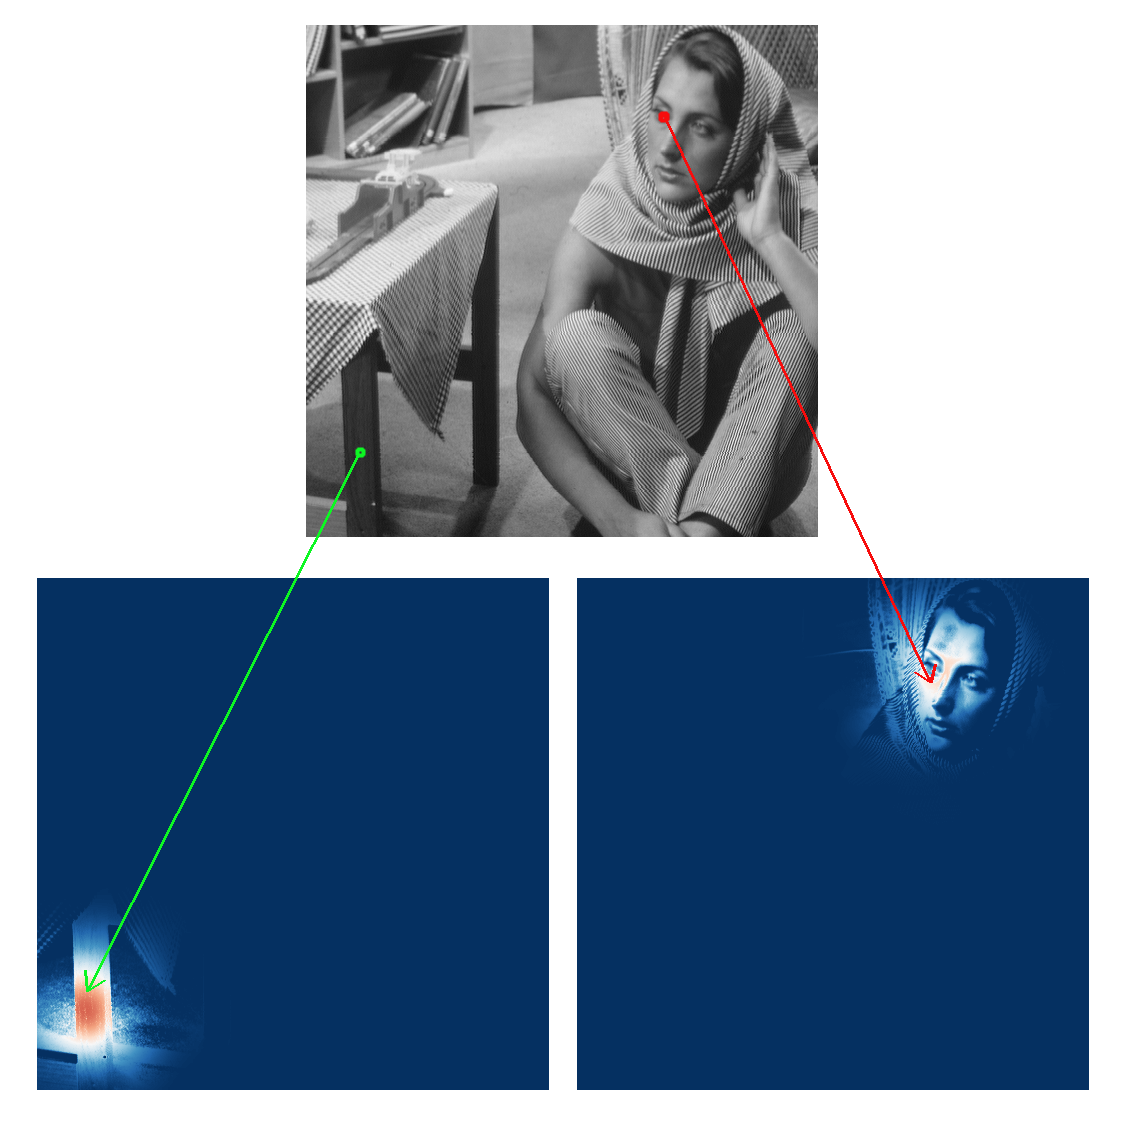
\includegraphics[width=\textwidth]{img/bilateralAffinityPhoto35Spatial50.png}
      \caption{Affinity matrices with \(h_x = 50\) and \(h_z = 35\)}
  \end{figure}
  In a very heterogeneous image, the bilateral kernel will be useful to keep the spatial similarity, but with excluding very dissimilar neighbour pixels.
  Remember that each matrix here is only one row of the affinity matrix.

 \item [Non-Local Means (NLM)] is similar to the bilateral kernel, a data-dependent filter, except that the photometric affinity is captured patch-wise \cite{glide_2014} \cite{kervrann_nlm_2006}.
 \item [Locally Adaptive Regression Kernel (LARK)] uses the geodesic distance based on estimated gradients \cite{milanfar_symmetrizing_2013} \cite{takeda_kernel_2007}.
\end{description}

\subsection{Graph Laplacian operator}

\paragraph{}
The graph Laplacian operator has multiple possible definitions and each has its own properties.
A good summary can be found in \cite{siam_slides_2016}.
A graph Laplacian can be symmetric which is important for the eigendecomposition of the matrix.
The spectral range, corresponding to the range of the eigenvalues, is important because we can use the filters derived from the Laplacian multiple times, and if the eigenvalues are not between 0 and 1, then the filters tend to be unstable.
With \(K\) being the affinity matrix, \(d_i = \sum_j K_{ij}\) and \(D = diag\{d_i\}\):

\begin{table}[!htbp]
 \centering
 \begin{tabular}{|c|c|c|c|c|}
  \hline
  Laplacian Name & Formula & Symmetric & Spectral Range \\
  \hline
  Un-normalised & \(D - K\) & Yes & [0, n] \\
  \hline
  Normalised & \(I - D^{-1/2}KD^{-1/2}\) & Yes & [0, 2] \\
  \hline
  Random Walk & \(I - D^{-1}K\) & No & [0, 1] \\
  \hline
  ``Sinkhorn" \cite{milanfar_symmetrizing_2013} & \(I - C^{-1/2}KC^{-1/2}\) & Yes & [0, 1] \\
  \hline
  Re-normalised \cite{milanfar_new_2016} & \(\alpha(D - K)\), \(\alpha = \bigO(N^{-1})\) & Yes & [0, n] \\
  \hline
 \end{tabular}
\end{table}
Generally, it is a good practice to stick to one definition of the Laplacian.

\section{Implementation}

\subsection{Algorithm details}
In our algorithm, we shall use spatially uniform sampling for the ease of implementation and robustness.
The kernel function is the bilateral one.

\subsection{Results}
TODO some results (image processing) + performances (for GMRES + ASM)


\chapter{Implementation}

\paragraph{}
This section presents the work that has been done on the implementation.
We start by touching a few words on which variations have been used and what has been done before implementing our algorithm in parallel.
After that, we explicit each step of the parallel implementation, what has been implemented by hand and the parts that come from a library.
Finally, we present our experiments, the results and discuss them.

\section{Algorithm details}

\paragraph{Variations}
In our algorithm, we use spatially uniform sampling for the ease of implementation and robustness.
The kernel function is the bilateral function with the spatial parameter \(h_x = 40\) and the color intensity parameter \(h_z = 20\).
We use the re-normalised Laplacian \(\Lapl = \alpha (D-K)\)from \cite{milanfar_new_2016} to avoid expensive computation and use a simple definition.

\paragraph{Prototyping}
Initially, we implemented the algorithm proposed by \cite{glide_2014} in Python, using Numpy, in order to understand the mechanisms and issues of global filtering.
After that, we wrote our adapted algorithm in Python again, as a quick proof of concept.
Needless to say that this implementation is sequential and limited to small images that require only little computational resources.

\section{Parallel implementation}

\paragraph{}
To scale our algorithm to use usual camera pictures, but also much larger inputs, we implemented it in a parallel manner using the C language and the Portable, Extensible Toolkit for Scientific Computation (PETSc) \cite{petsc_web_page}.
This library is built upon MPI and contains distributed data structures and parallel scientific computation routines.
The most useful are the matrix and vector data structures and the parallel matrix-matrix and matrix-vector products.
Additionally, PETSc provides Krylov subspace methods and preconditioners for solving linear systems, also implemented in a scalable and parallel manner.
In a nutshell, PETSc provides an impressive parallel linear algebra toolkit, very useful to shorten the development time.
As we are basically using MPI, the main parallelism technique that we apply is SPMD.
It is possible to activate some SIMD parallelism with PETSc but we do not consider it in our case.
We want to point out to the reader that the distributed PETSc matrix data structure splits the data without overlap in a row-wise distribution manner.
In order to verify the correctness of our implementation, we used the Scalable Library for Eigenvalue Problem Computation (SLEPc) \cite{hernandez_slepc_2005}, which is based on PETSc and provides parallel eigenvalue problem solvers.
Furthermore, we need the library Elemental \cite{poulson_elemental_2013} in order to achieve dense matrix operations in PETSc.

We present how we included parallelism in our algorithm step-by-step, starting with reading the image and sampling.
Then follows the computation of the affinities of the sampled pixels.
And we finish with the computation of the smallest eigenvalues using the inverse subspace iteration.
The implementation associated to this project is open source and can be found on GitHub\footnote{\url{https://github.com/David-Wobrock/image-processing-graph-laplacian/}}.

\paragraph{Initialisation and sampling}
During the initialisation phase, the input image is read into memory sequentially by process 0.
Since we consider that the input image fits into memory, we broadcast the entire image from process 0 to all other processes.
Every process will hold the entire input image which will be useful since every process needs every pixel to compute the affinities.

The sampling step is also done by every process independently in a deterministic way.
All processes know the indices of the sampled pixels.
This is possible because we use spatially uniform sampling, which is deterministic, fast to compute and doesn't require communication.

\paragraph{Submatrices computations}
The computation of the affinity submatrices \(K_A\) and \(K_B\) is done locally by each process.
Indeed, each process computes the rows of the matrix that it will hold locally.
In other words, each process computes the affinities between a continuous subset of the sampled pixels and all pixels.
Since every process holds the complete image, no communication is needed.
The overhead is thus minimal and this part of the algorithm scales very well with respect to the number of processes.

Then, we compute the Laplacian submatrices \(\Lapl_A\) and \(\Lapl_B\).
The submatrix \(\Lapl_A\) requires to first compute the part \(D_A\) of the diagonal matrix \(D\) of normalisation coefficients.
Again, each process can locally sum each row of \(K_A + K_B\) because they have the same distribution layout, so no communication is needed.
However, to compute the normalisation factor \(\alpha\) in our Laplacian definition \(\alpha (D - K)\) with \(\alpha = \bar{d}^{-1}\) and \(\bar{d} = \sum^N_{i=1} \frac{d_i}{N}\), we need communication to find the average of the normalisation coefficients.
Nevertheless, the implied communication costs are not critical since we broadcast only one value for each process.

\paragraph{Inverse subspace iteration}
The algorithm to compute the smallest eigenvalues we use is the inverse subspace iteration inspired by \cite{el_khoury_acceleration_2014}.
With \(m\) the number of eigenvalues we will compute, \(p\) the sample size and \(m \le p\), we start the algorithm by selecting \(m\) random orthonormal independent vectors \(X_0\) of size \(p\).
We implemented a parallel Gram-Schmidt orthonormalising routine, based the classical sequential one.

The inverse iteration algorithm consists of outer and inner iterations, with \(k\) the index of the current outer iteration index.
The inner iteration consists of solving \(m\) linear systems, one for each vector of \(X_k\) that we approximate, such that \(\forall i \in [1, m]\) and \(X_k^{(i)}\) the \(i\)th vector of the subspace \(X_k\):
\[A X_{k+1}^{(i)} = X_k^{(i)}.\]
The outer iteration consists of repeating this process until convergence, meaning having a small enough residual norm.
We define the residual \(R_k\) of \(X_k\), at a certain iteration \(k\), as
\[R_k = A X_k - X_k X_k^T A X_k = (I - X_k X_k^T) A X_k.\]
A summary of the inverse subspace iteration algorithm:

\begin{algorithm}[H]
 \caption{Inverse subspace iteration}
 \begin{algorithmic}
  \REQUIRE \(A\) the matrix of size \(p \times p\), \(m\) the number of required eigenvalues, \(\varepsilon\) required precision of the subspace
  \ENSURE \(X_k\) the desired invariant subspace
  \STATE Initialise \(m\) random orthonormal vectors \(X_0\) of size \(p\)
  \STATE For k=0, 1, 2, \dots
  \WHILE{\(\|R_k\| > \varepsilon\)}
   \FOR{i=1 \TO m}
    \STATE Solve \(A X_{k+1}^{(i)} = X_k^{(i)}\)
   \ENDFOR
   \STATE Orthonormalise \(X_{k+1}\)
  \ENDWHILE
 \end{algorithmic}
\end{algorithm}

Solving the systems of linear equations is done using the Krylov type solvers and the preconditioners included in PETSc.
As a standard approach, we use the Restricted Additive Schwarz (RAS) method as preconditioning method, without overlap and 2 domains per process.
Each subdomain is solved using the GMRES method.

On each outer iteration, we must compute the residuals to see if we converged.
This is requires multiple matrix-matrix products and computing a norm, so communication cannot be avoided here.

\paragraph{Nystr\"om extension and output image}
As stated before, the Nystr\"om extension finds the leading eigenvectors, whereas we would need the trailing ones, as explains the articles \cite{belongie_spectral_2002}, \cite{fowlkes_spectral_2004} and \cite{glide_2014}.
So the algorithm will not compute the output image for now.

\section{Results}

\paragraph{Experimental setup}
The experiments to see how the algorithm scales are done on the test supercomputer of the Laboratoire Jacques-Louis Lions at Sorbonne Université.
This computer has 32 CPUs of 10 cores each and a total memory of 2 TB.
The setup of the experiments consists of running a specific test with different parameters, scaling the algorithm up to 250 processors.
The code is compiled on this computer using GCC 6.3.0 and the MPI implementation is Open MPI 1.8.3.
The versions of other libraries are PETSc 3.8.3, SLEPc 3.8.2 and Elemental 0.87.7.

\paragraph{}
We start by executing the algorithm without approximation.
This way, we will be able to see the results of the algorithm, even if the size of the input images will be limited.
After that, we study the approximation and computation of the smallest eigenvalues of the Laplacian.

\subsection{Entire matrix computations}

\paragraph{Results}
We start by showing the result of the computation using the full matrices.
We limited ourselves to grayscale images for the beginning and for computing the entire matrices, we can only process small images.
The image below is of size \(350 \times 350\), 122 500 pixels, so each matrix taking around 120 GB.

\begin{figure}[H]
  \centering
  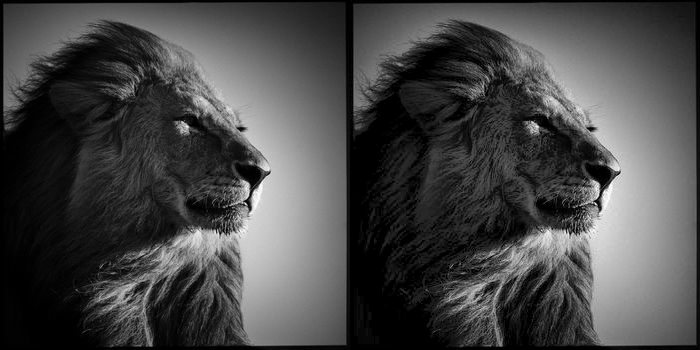
\includegraphics[width=0.95\textwidth]{img/lion.png}
  \caption{Left: input image. Right: sharpened image.}
\end{figure}

We observe more details on the lion's head and the mane on the left-hand side appears brighter.
However, the already detailed parts are not over-sharpened.
The sharpening is done by defining the output image as \(z = (I - f(\Lapl))y\) with, in this case, \(f(\Lapl) = -3\Lapl\).
We fall back on the adaptive sharpening operator defined in \cite{siam_slides_2016} as \((I + \beta \Lapl)\) with \(\beta > 0\).

\paragraph{Performances and discussions}
We run the algorithm 5 times for each number of processors, on the image shown above, from 8 to 128 processors for each power of 2.
First, the total runtime for each number of processors:
\begin{figure}[H]
  \centering
  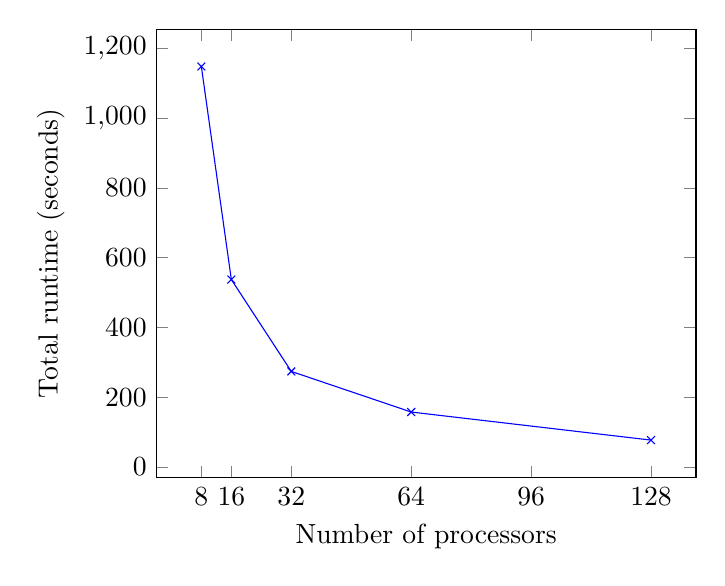
\begin{tikzpicture}
   \begin{axis}[
    xlabel=Number of processors,
    xtick={8, 16, 32, 64, 96, 128, 150},
    ylabel=Total runtime (seconds)]
     \addplot[color=blue, mark=x] coordinates {
      (8, 1148.389)
      (16, 537.521)
      (32, 274.0227)
      (64, 157.5765)
      (128, 77.0977)
     };
   \end{axis}
  \end{tikzpicture}
  \caption{Total runtime of the algorithm with entire matrix computation.}
\end{figure}

We observe that the runtime decreases significantly with respect to the number of processors.
We can also see that, by doubling the number of processors, we nearly accelerate the runtime by a factor 2.
It is one of the best result we could expect since we achieved strong scalability for the entire matrix computation case.
However, some overhead will always be present and the matrix-vector operations necessarily require communication, limiting scalability.
To observe if some parts scale better than others, we compare the proportion of each part:
\begin{figure}[H]
  \centering
  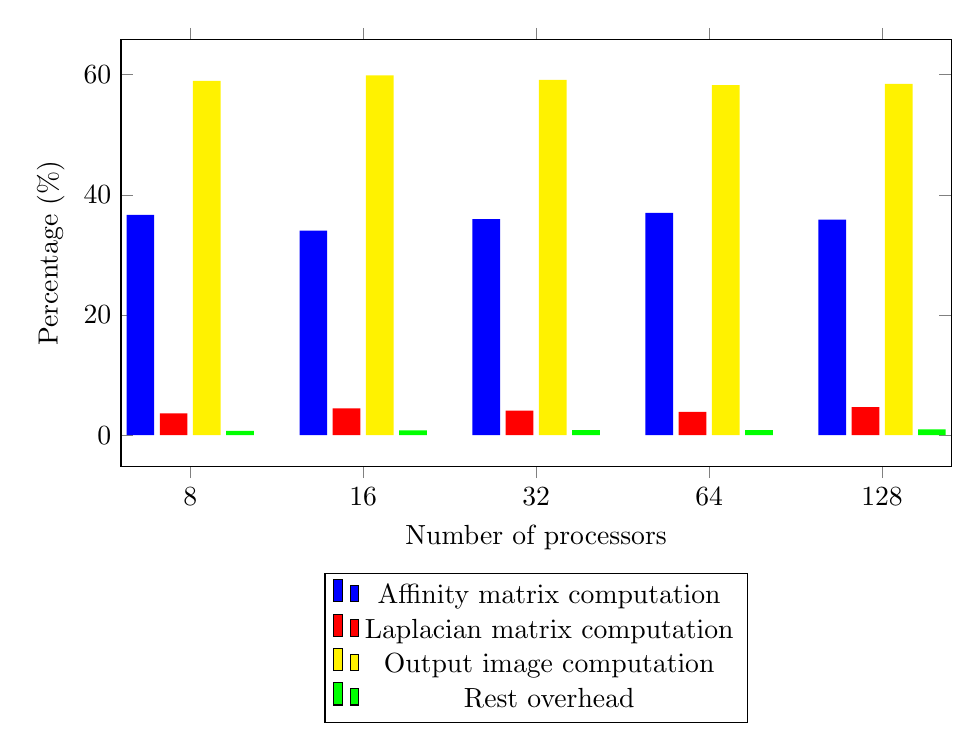
\begin{tikzpicture}
   \begin{axis}[
    ybar,
    height=7cm,
    width=\textwidth,
    xlabel=Number of processors,
    xtick={0, 1, 2, 3, 4},
    xticklabels={8, 16, 32, 64, 128},
    legend style={
     at={(0.5, -0.25)},
     anchor=north
    },
    ylabel={Percentage (\%)}]
    \addplot[draw=none, fill=blue] coordinates {
     (0, 36.67)
     (1, 34.04)
     (2, 35.96)
     (3, 37)
     (4, 35.88)};
    \addplot[draw=none, fill=red] coordinates {
     (0, 3.62)
     (1, 4.48)
     (2, 4.07)
     (3, 3.88)
     (4, 4.67)};
    \addplot[draw=none, fill=yellow] coordinates {
     (0, 58.99)
     (1, 59.9)
     (2, 59.15)
     (3, 58.26)
     (4, 58.48)};
    \addplot[draw=none, fill=green] coordinates {
     (0, 0.72)
     (1, 0.78)
     (2, 0.82)
     (3, 0.86)
     (4, 0.96)};
    \legend{Affinity matrix computation,
     Laplacian matrix computation,
     Output image computation,
     Rest overhead}
   \end{axis}
  \end{tikzpicture}
  \caption{Proportion of each step in the total execution of the algorithm with entire matrix computation.}
\end{figure}

We see that the proportion of each part remains the same, meaning that the three main parts, in this interval of number of processors, scale equivalently.
When allocating an excessive amount of processors to this task, it may be that we observe an increase of the runtime because we spend time communicating.

\subsection{Approximation computations}

\paragraph{Eigenvalues}
We remind that the end of the algorithm, using matrix approximations to compute the filtered image, is not implemented.
Nonetheless, we will present interesting results about the computation of the eigenvalues of the graph Laplacian operator.

\paragraph{Performances}
TODO

\paragraph{SLEPc comparison}
TODO


\chapter{Conclusion}

\section{Discussions}
\paragraph{Linear solvers \& domain decomposition methods on dense matrices}
The presented experiments show that the resolution of linear systems scales with respect to the number of processors.
Domain decomposition methods improve the performances of solving dense systems of linear equations, even without overlap, in the context of image processing.
Indeed, these methods are naturally parallel and precondition the matrix appropriately.
This becomes clear when observing the performances improvement on large matrices.

\ifthesis
 In the case of a small input image, a direct solver shows the best results for computing the inverses for preconditioning.
 On larger inputs, these are not available but using iterative Krylov type methods on the subdomains also exposes a considerable improvement compared to the case without preconditioner.
\fi

\paragraph{Gram-Schmidt process}
The orthogonalisation process is difficult to parallelise efficiently.
\ifthesis
 Skipping the Gram-Schmidt procedure every other iteration, to stabilise the algorithm less often, gave an improvement, but we cannot totally avoid the cost of it when increasing the number of processors.
 Skipping the Gram-Schmidt procedure more often tends to improve the runtime when a large amount of processors is involved.
\else
 Skipping the Gram-Schmidt procedure tends to improve the runtime when a large amount of processors is involved.
\fi
However, the stability of the algorithm diminishes when omitting numerous orthogonalisations.
This scalability problem is well-known and one of the biggest limitations for scaling diverse algorithms to a large number of processors.

The Gram-Schmidt procedure orthogonalises a set of vectors by sequentially substracting from a vector the projections on the previously orthogonalised vectors.
The inner product of two vectors is computed frequently, because of the projection, and since each vector is shared over all processors, a lot of communication is involved in this operation.
Attempts for parallel implementation are numerous, like \cite{katagiri_parallel_gram_schmidt_2003}, but they either still have many communications or suggest a different memory distribution schema.


\section{Perspectives}
\paragraph{Image processing}
Numerous possibilities for improving the algorithm result from the applied simplifications.
An important matter would be to complete the final part of the algorithm computing the output image.
This requires to compute the inverse of the square root of the matrix.
\ifthesis
 This can be done either by calculating the entire eigendecomposition to get the inverse square root matrix.
 Another way to accomplish this, could be to consider Cauchy's integral formula such as:
 \[A^{-\frac{1}{2}} = \frac{1}{2\pi i} \oint_C z^{-\frac{1}{2}} (zI - A)^{-1} \mathrm{d}z.\]
 However, the time for this project was not sufficient to explore this possibility entirely.

 An easy improvement to make such an algorithm production ready, would be to consider color images.
 This can be done by decomposing the RGB image to a YCC image, with one grayscale and two chroma components.
 The algorithm is applied to all three components, and then they are converted back to RGB.
\fi

A way to improve the filtering is multiscale decomposition.
As explained in \cite{talebi_nonlocal_2014}, instead of applying a linear function to all eigenvalues such as \(f(W) = \phi f(\Pi) \phi^T\), we can actually use a polynomial function \(f\).
This is interesting because each eigenpair captures various features of the image and one can apply different coefficients on different aspects of the image.

For the state-of-the-art, the article \cite{talebi_fast_2016} proposes an enhancement of global filtering.
They argue that the eigendecomposition remains computationally too expensive and show results of an improvement.
The presented results and performances are astonishing; however, the method is hardly described and replicating it would be difficult.
This is understandable since this algorithm seems to be in the latest Pixel 2 smartphone by Google and they surely want to preserve their market advantage in the field of image processing.

\paragraph{}
An improvement of the algorithm of the present case, would be to formulate a method for extending the trailing eigenvectors of the sampled Laplacian \(\Lapl_A\) and not only the leading ones as the Nystr\"om extension supports.
This way, it would be possible to apply the spectral decomposition of the Laplacian, and thus apply a filter to the input image, avoiding the computation of the inverse square root of the matrix.

\ifthesis
 \paragraph{Linear solver}
 A way to highly parallelise the matrix computations could be using graphical processing units (GPUs).
 Especially the matrix-matrix and matrix-vector products could be nicely improved with GPUs.
 However, solving systems of linear equations is a task that GPUs are not designed for.

 \paragraph{}
 It also would be interesting to explore more the impact of the number of sampled pixels, which corresponds to the input matrix of the linear system.
 The articles \cite{fowlkes_spectral_2004} and \cite{glide_2014} started a study on the size of the samples, but only for small images.
 This work could be extended.
\fi

To conclude, various possibilities remain to be exploited by future work.



\clearpage
\printbibliography

\appendix % appendix

\chapter{Proof of filter and Laplacian eigenvalues equivalence}
\label{appendix:eigenvalue_proof}
\paragraph{}
The filter \(W\) is built on top of the kernel matrix \(K\) measuring the similarity between each pixel.
The most popular kernel functions are the \textit{bilateral filter} \cite{bilateral_tomasi_1998} and the \textit{non-local mean filter} \cite{kervrann_nlm_2006} to measure these similarities.
The kernel functions create a symmetric positive semi-definite (SPSD) matrix \(K\), so the eigenvalues of \(K\) are non-negative, \(\lambda_K \ge 0\), as described in \cite{talebi_fast_2016}.
Also, from the definition of the filters, \(\forall i, j \in [1, N]\), \(N\) the number of pixels, the values of the affinity matrix \(K\) are non-negative \(K_{ij} \ge 0\).

\paragraph{}
Without loss of generality, we shall use a Laplacian operator that is symmetric positive definite (SPD) by definition.
The filter is implicitely defined by \cite{modern_tour_2013} as \(W = I - \Lapl\) and if the Laplacian eigenvalues are between 0 and 1, so are the eigenvalues of \(W\).

We can say that for a principal submatrix \(W_A\) of size \(p \times p\) of the matrix \(W\) of size \(N \times N\) with \(p \ll N\), the eigenvalues \(\lambda^W_i \le \lambda^{W_A}_i \le \lambda^W_{i+N-p}\).
This is the interlacing property, meaning in general, \(\lambda^W_1 \le \lambda^{W_A}_i \le \lambda^W_N\).

\paragraph{Proof of interlacing}
Let \(A\) be a symmetric matrix of size \(n\), \(\lambda^A_n\) be the largest eigenvalue of \(A\) and \(\lambda^A_1\) the smallest one.
Let \(R\) be the restriction operator, such as, with \(u\) a non-zero vector, \(Ru = \begin{pmatrix}\alpha_1 \\ \alpha_2 \\ \vdots \\ 0 \\ \vdots \\ 0 \end{pmatrix}\) for example.
This defines \(RAR^T\) a \(s \times s\) principal submatrix of \(A\) with  \(s \in [1; n]\).
Suppose the remaining rows and columns of \(A\) in \(RAR^T\) are indexed by \(S\) of size \(s\). \\
Let \(\mathcal{U} \in \Real^s\) and \(u \in \Real^n\) with \(\begin{cases} u_i = \mathcal{U}_i & \quad \text{if } i \in S \\ u_i = 0 & \quad \text{if } i \notin S \end{cases}\).
Given a \(k \in [1; s]\), the Courant-Fischer theorem, involving the Rayleigh-Ritz quotient, implies that,
\[max\left(\frac{\langle Au, u \rangle}{\langle u, u\rangle}\right) = max\left(\frac{\langle RAR^T\mathcal{U}, \mathcal{U}\rangle}{\langle \mathcal{U}, \mathcal{U} \rangle}\right) \ge \lambda^A_k.\]
So \(\lambda^{RAR^T}_k \ge \lambda^A_k\).
More over, in the other way, we get
\[min\left(\frac{\langle Au, u \rangle}{\langle u, u\rangle}\right) = min\left(\frac{\langle RAR^T\mathcal{U}, \mathcal{U}\rangle}{\langle \mathcal{U}, \mathcal{U} \rangle}\right) \le \lambda^A_{k+n-s}.\]
And so again, \(\lambda^{RAR^T}_k \le \lambda^A_{k+n-s}\).
This concludes the proof, showing that the eigenvalues of the submatrix are bounded by the eigenvalues of the original matrix.
More precisely, we proved the interlacing property of the eigenvalues of \(RAR^T\) such as
\[\lambda^A_k \le \lambda^{RAR^T}_k \le \lambda^A_{k+n-s}.\]

\paragraph{}
From the definition of the filter \(W = I - \Lapl\), we have the submatrix \(W_A = I - \Lapl_A\), with \(I\) being the identity of appropriate order.
For the algorithm, we need to compute the largest eigenvalues of \(W_A\).

\paragraph{Theorem}
Computing the largest eigenvalues of \(W_A\) is equivalent to computing the smallest eigenvalues of \(\Lapl_A\).

\paragraph{Proof}
Let \(\lambda\) be an eigenvalue of \(W_A\) and \(x\) the associate eigenvector:
\begin{equation}
 \begin{split}
     W_A x = \lambda x & \Leftrightarrow (I - \Lapl_A)x = \lambda x \\
                     & \Leftrightarrow x - \Lapl_A x = \lambda x \\
                     & \Leftrightarrow \Lapl_A x = x - \lambda x \\
                     & \Leftrightarrow \Lapl_A x = (1 - \lambda) x
 \end{split}
\end{equation}
So the eigenvalues of the Laplacian submatrix \(\mu = 1 - \lambda\).
We can thus get the greatest eigenvalues of \(W_A\) by computing the smallest eigenvalues of \(\Lapl_A\).

\paragraph{Speed of convergence}
For both these problems, finding the greatest and smallest eigenvalues, the most famous methods are, respectively, the power method and inverse power method\footnote{Those are also called power iteration and inverse iteration. The inverse method has a variant called inverse subspace iteration, to find the associated subspace to the eigenvalues.}.

For the power iteration, the convergence rate is \(|\frac{\lambda_2}{\lambda_1}|\), with \(\lambda_2\) being the second largest eigenvalue.
We know that \(\lambda^{W_A}_2 \le \lambda^{W_A}_1 \le 1\) and thus \(\frac{\lambda^{W_A}_2}{\lambda^{W_A}_1} \le \frac{\lambda^{W_A}_1}{\lambda^{W_A}_1} = 1\).
The convergence rate is lower than 1.
The method is fast if the rate is small and slow if the rate is close to 1.
So the closer the two eigenvalues are, the slower the method converges.

The inverse iteration has a speed of convergence of \(|\frac{\mu_1}{\mu_2}|\), with \(\mu_2\) the second smallest eigenvalue.
Again, we know that \(0 \le \mu^{\Lapl_A}_1 \le \mu^{\Lapl_A}_2\).
So the convergence speed is also lower than 1.

We come to the conclusion that both methods depend on the spacing between the eigenvalues.
The closer they are, the more iterations will be required to converge.
The difference of convergence speeds for both methods therefore depends on the distance between the largest eigenvalues and the distance between the smallest ones.

\paragraph{}
Inverse iterations implies either to compute the inverse of the matrix \(x_{k+1} = A^{-1}x_k\), or to solve a system of linear equations \(Ax_{k+1} = x_k\).
Since the image processing context suggests having dense matrices, we want to explore the performances of Krylov methods and domain decomposition methods (e.g. the Additive Schwarz method) on such dense matrices.


\end{document}
